\documentclass[12pt]{article}
\usepackage[a4paper, left=3cm, right=3cm]{geometry}	% Per i margini
\usepackage[latin1]{inputenc}
\usepackage{amssymb}
\usepackage{color, xcolor}
\usepackage{graphicx}	% Per immagini e pdf.
\usepackage{amsmath}
\usepackage{subfigure}

\title{Progetto di Sistemi per il Governo dei Robot mod. A}
\author{Riccardo Grieco, Marco Matarese, Andrea Pollastro}

\begin{document}
	%\maketitle
	% --- TITLE PAGE --- %

\thispagestyle{empty}

\begin{center}
	
\includegraphics[width=0.8\textwidth]{images/DIETI}\\
	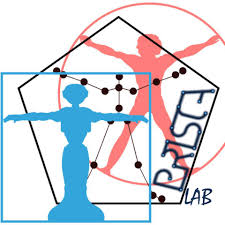
\includegraphics[width=0.2\textwidth]{images/prisca.jpg}
	
	\par\bigskip\par\bigskip\par\bigskip
	%\par\bigskip\par\bigskip\par\bigskip\par\bigskip\par\bigskip\par\bigskip\par\bigskip\par	% Per spazi
	
	{\huge Touch the Color\\}
	%{\huge Algoritmi e Strutture Dati II\\}
	
	\par\bigskip\par\bigskip\par\bigskip\par\bigskip\par\bigskip\par\bigskip\par\bigskip\par	% Per spazi
	
	{\LARGE Progetto di \\}
	{\LARGE Sistemi per il Governo dei Robot mod. A\\}
	{\large A.A 2018/2019\par}
	
	\par\bigskip\par\bigskip\par\bigskip\par\bigskip\par\bigskip\par\bigskip
	
	{\large Grieco Riccardo N97/28 \\}
	{\large Matarese Marco N97/280 \\}
	{\large Pollastro Andrea N97/28 \\}
	
	\par\bigskip\par\bigskip\par\bigskip\par\bigskip\par\bigskip\par\bigskip	
	
	
	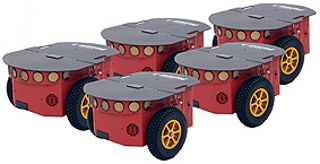
\includegraphics[width=0.3\textwidth]{images/pioneer.jpg}
\end{center}

	\newpage
	
	\tableofcontents
	
	\newpage
	
	\section{Introduzione}
		%	INTRODUZIONE


\subsection{Descrizione del Gioco}
Touch the color, o "Strega chiama color" nella sua versione italiana, � un semplice gioco di gruppo da svolgersi all'aria aperta. Questo prevede la selezione di un giocatore del gruppo al ruolo di strega, il quale dovr� scegliere un colore ed urlarne il nome a tutti gli altri componenti del gruppo. Quest'ultimi, udito il colore, dovranno cercare nel minor tempo possibile un oggetto del colore indicatogli per poi raggiungerlo: l'ultimo giocatore a "toccare il colore" verr� selezionato come strega al prossimo giro.

\subsection{Nicchia Ecologica}

\subsection{Schema dei Behaviours}

		\clearpage
		
	\section{Navigazione}
		Per la navigazione del robot, in particolare del robot \textit{Kid}, � stato utilizzato un approccio misto che utilizza sussunzione e metodologia a campi di potenziale.

\subsection{Campi di potenziale}
	I campi previsti dall'architettura sono i seguenti:
	\begin{itemize}
	    \item Wander
	    \item Avoid
	    \item Move To Goal
	\end{itemize}
	Le forze esercitate dai campi di potenziale hanno per convenzione intensit� nell'intervallo $[0,1]$. \\
	 \\
	Il campo Wander, che permette l'esplorazione dell'ambiente, applica al robot una forza costante in avanti rispetto al suo orientamento. 
	Con cadenza costante, il campo genera una forza con un orientamento rispetto al sistema di riferimento del robot tra i -90� e i +90� in maniera casuale. %TODO sicuro?
	Il vettore generato ha la massima intensit� possibile.
	% Plot del campo Avoid
	\begin{figure}[h!]
		\centering
		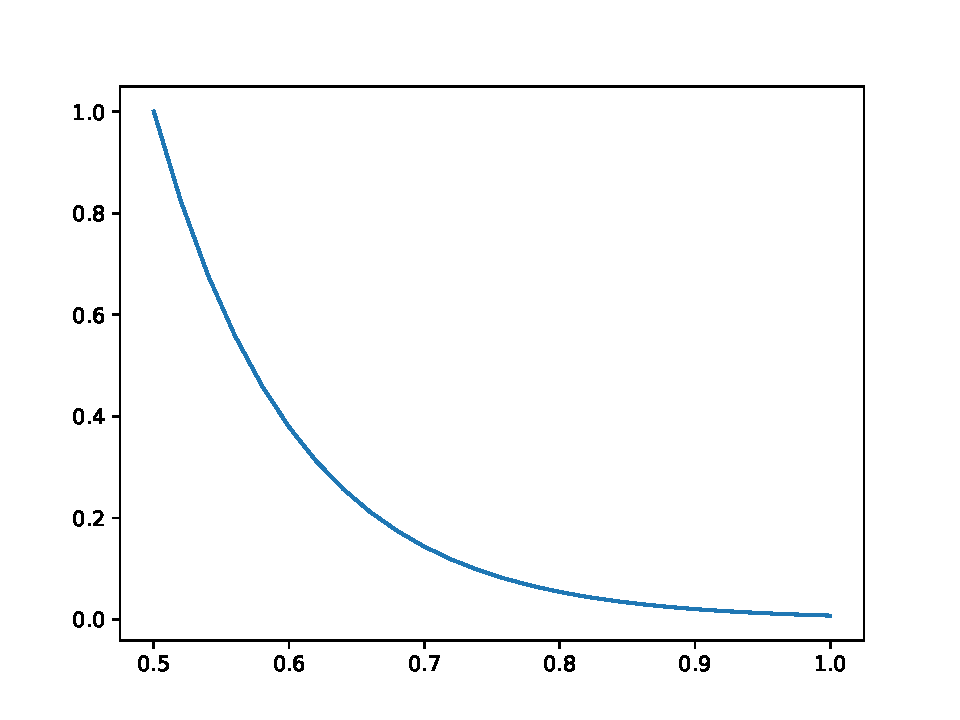
\includegraphics[width=0.7\textwidth]{images/repulsionplot.pdf}
		\caption{Plot della funzione del campo Avoid. Sull'asse delle ascisse troviamo la distanza dall'ostacolo, su quello delle ordinate l'intensit� del campo repulsivo.}
		\label{fig:repulsion_plot}
	\end{figure}
	\newpage
	Il campo Avoid permette la \textit{Obstacle Avoidance}. Ogni ostacolo genera un campo repulsivo con un profilo di ampiezza esponenziale. In particolare, l'intensit� della forza generata dal campo segue la funzione:
	\begin{center}
		$avoid(d) = b^{-c (d-D_S)} $
	\end{center}
	dove $d$ � la distanza del robot dall'oggetto, $b$ e $c$ sono fattori che determinano il comportamento della curva e $D_S$ � una distanza di sicurezza, fissata a priori.
	Il campo viene percepito solo quando la distanza dall'oggetto � di almeno 1 metro.
	La Figura~\ref{fig:repulsion_plot} evidenzia come la forza esercitata dal campo abbia intensit� massima quando l'oggetto si trova ad una distanza vicina quella di sicurezza e minima al limite della percezione del campo.\\ \\
	%Plot del campo Move to Goal
	\begin{figure}[h!]
		\centering
		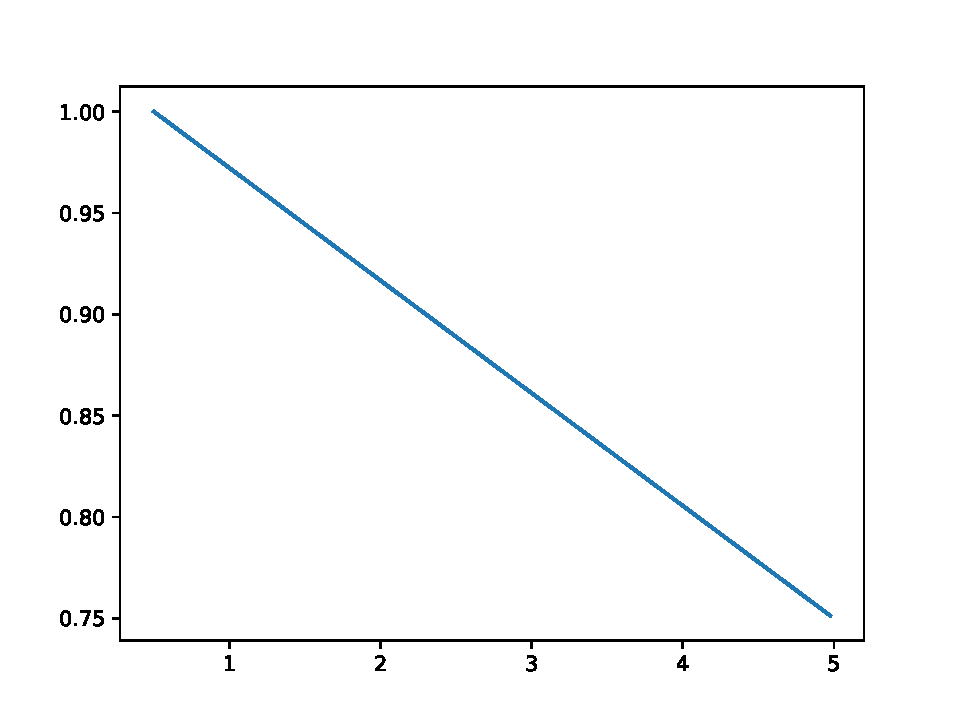
\includegraphics[width=0.7\textwidth]{images/attractionplot.pdf}
		\caption{Plot della funzione del campo Move to Goal. Sull'asse delle ascisse troviamo la distanza dall'ostacolo, su quello delle ordinate l'intensit� del campo attrattivo.}
		\label{fig:attraction_plot}
	\end{figure}

	Il campo Move to Goal permette al robot di raggiungere un punto di interesse che, nel caso in esame, � il colore a cui avvicinarsi. Il punto di interesse (POI) genera un campo attrattivo di intensit� lineare sulla distanza dal robot. Questo segue la seguente funzione:
	\begin{center}
		$attract(d) = \frac{1-F_{min}}{D_S-D_A} (d-D_S)+1$
	\end{center}
	dove $F_{min}$ � la minima intensit� garantita dal campo mentre $D_S$ e $D_A$ sono rispettivamente la distanza di sicurezza e la minima distanza di percezione del campo.
	Il campo viene percepito solo quando l'oggetto si trova ad una distanza affidabile, ovvero tale per cui il riconoscimento dello stesso ha una certa affidabilit�. Nel caso in questione, in cui il punto di interesse viene riconosciuto da una telecamera RGB-D, la rilevazione � affidabile quando l'oggetto si trova ad una distanza di al pi� 5 metri.
	La Figura~\ref{fig:attraction_plot} mostra come la forza esercitata dal campo abbia intensit� massima quando l'oggetto si trova vicino al POI, mentre a distanza massima di percezione garantisca comunque un'intensit� abbastanza elevata, permettendo al robot di raggiungere il punto di interesse pi� o meno velocemente.

\subsection{Orientamento}
	Il sistema di coordinate utilizzato � robocentrico, ovvero ogni punto rilevante (ostacoli, punto di interesse) nello spazio � individuato da coordinate ottenute dalle misurazioni dei sensori che il robot utilizza.\newline Questo sistema rende molto facile l'utilizzo dei campi di potenziale per l'individuazione di un vettore che determini il movimento del robot.
	Un problema che sorge dall'utilizzo di questo sistema � quello di gestire punti di cui non si hanno pi� rilevazioni dai sensori. Nel caso specifico del robot Kid, se esso non ha pi� visibilit� del POI che cerca di raggiungere, ad esempio perch� si � dovuto girare per evitare un'ostacolo, dovrebbe comunque poter stimare la posizione dell'oggetto.
	Per fare ci� � necessario memorizzare lo spostamento e la rotazione effettuati dal sistema di riferimento rispetto all'ultima volta in cui tale oggetto � stato rilevato.
	Ottenere questi dati � possibile grazie all'utilizzo dell'interfaccia RosAria per la gestione della mobilit� del robot. Il nodo ROS RosAria pubblica sul topic \texttt {/RosAria/pose} le informazioni sulla posizione e sull'orientamento del robot. I messaggi pubblicati sul topic utilizzano un sistema di coordinate mondocentrico, in cui orientamento e origine coincidono con l'orientamento e la posizione del robot al momento dell'avvio del nodo RosAria.
	Per calcolare lo spostamento e la rotazione effettuata dal robot, basta memorizzare le informazioni pubblicate sul topic al momento dell'ultima rilevazione del punto di interesse e le informazioni "attuali" fornite da RosAria.
	Il vettore di traslazione e la matrice di rotazione sono calcolati come segue:
	\begin{center}
		$t = (p_s - p_c) R_s$
	\end{center}
	
	\begin{center}
		$R = 
		\begin{bmatrix}
			\cos(\theta) & -\sin(\theta) \\
			\sin(\theta) & \cos(\theta)
		\end{bmatrix}$
	\end{center}
	dove $p_s$ e $p_c$ sono  rispettivamente la posizione al momento dell'ultima rilevazione dell'oggetto di interesse e la corrente. $R_s$ � la matrice di rotazione al momento dell'ultima rilevazione del POI e $\theta$ � l'ampiezza dell'angolo di cui � ruotato il robot rispetto all'ultima rilevazione.\\
	\newpage
	Il punto di interesse, una volta fuori dal campo visivo del robot, viene calcolato come segue %TODO
	\begin{center}
		$POI_c = (POI_s + t) R$
	\end{center}
	dove $POI_s$ � la posizione del punto di interesse al momento dell'ultima rilevazione.
\subsection{Movimento} %TODO ??
	Lo schema motorio � costituito da un'unica funzione \texttt{move}, che decide il movimento del robot in base alla forza complessiva esercitata dai campi di potenziale. La coordinata x della forza determina la rotazione del robot, mentre la y determina l'intensit� del movimento in avanti.
	La velocit� lineare e quella angolare, data la forza $F$, sono cos� rispettivamente  calcolate:
	\begin{center}
		$v = \frac{F_y}{4}$
	\end{center}
	\begin{center}
		$\omega = \frac{F_x}{2}$
	\end{center}
	In questo modo la velocit� lineare massima raggiunta � di $0.25$ $m/s$ mentre quella angolare assume un valore massimo di $1.57$ $rad/s$ ($90�/s$).
	
		\newpage
		
	\section{Modulo per la Comunicazione}
		%	MODULO PER LA COMUNICAZIONE
% socket
% passaggio ip
% protocollo comunicazione

La comunicazione fra i robot � stata implementata tramite socket tcp. Tale tecnologia ci ha permesso, tramite la conoscenza pregressa degli indirizzi IP di tutti i robot partecipanti, di costruire delle linee di comunicazione punto-punto. Come gi� visto nella sezione introduttiva, il gioco prevede due ruoli: sono proprio i giocatori di ruoli diversi i soli a doversi scambiare messaggi.

\subsection{Gestione delle Socket}

Ogni robot gestisce almeno una socket: il Role Manager del nodo Witch ne gestisce una per ogni robot Kid e i Role Manager dei nodi Kid ne gestiscono una soltanto. Le socket, a prescindere dalla tipologia di nodo, vengono gestite attraverso il metodo \texttt{manageSocket(threadSocket)} della classe \texttt{RoleManager}. Il metodo in questione prende in input il file descriptor della socket su cui si metter� in ascolto e a cui invier� messaggi. \texttt{manageSocket} viene eseguito da un thread a parte, generato nel metodo \texttt{createAndStartConnection} solo per questo compito. In particolare, abbiamo che i nodi Kid generano un solo nuovo thread e il nodo Witch genera un thread per ogni nodo Kid a cui deve connettersi. Tale metodo non fa altro che rimanere in ascolto della socket passatagli finch� la variabile d'istanza \texttt{stopThread} non viene settata a \texttt{true}: ci� accade quando la partita in corso � terminata e bisogna resettare i parametri della classe \texttt{RoleManager}. I messaggi che arrivano sulla socket vengono quindi intercettati all'interno di questo loop e gestiti da un \textit{handler} di funzioni - implementato attraverso un array di riferimenti a funzioni - il quale, a seconda del tipo di messaggio ricevuto, invoca il metodo responsabile della gestione di quest'ultimo. Una volta usciti dal "loop di ascolto" il thread in questione viene fermato. 

ROS permette la definizione di variabili globali al sistema, referenziabili a run-time dai diversi nodi. Abbiamo scelto di sfruttare questa possibilit� offerta da ROS per comunicare ai robot gli indirizzi IP di tutti i partecipanti, incluso il proprio. I primi memorizzati in una lista di stringhe e il secondo in una semplice stringa, queste variabili vengono settate una volta sola (dopo aver eseguito \textit{roscore}) attraverso le due istruzioni seguenti e recuperate nel metodo \texttt{\_\_init\_\_} del nodo \texttt{RoleManager}.
\begin{center}
	\texttt{setparam /ipList "['100.101.0.10', '100.101.0.11', '100.101.0.11']"}
	\texttt{setparam /myIPAddress "100.101.0.10"}
\end{center}

\subsection{Il Protocollo di Comunicazione}

	Il protocollo di comunicazione � molto semplice: la struttura statica del gioco ci ha permesso di definire un protocollo rigido. I messaggi vengono scambiati solo tra giocatori di ruoli diversi, in particolare tra i Kids e la Witch: questo spiega la scelta di collegamenti punto-punto delle socket.
	
	Sono stati previsti tre tipi di messaggio:
	\begin{itemize}
		\item un messaggio in cui la Witch comunica a tutti i Kids il colore da toccare, dando cos� il via al gioco;
		\item un messaggio in cui un Kid comunica alla Witch di aver appena toccato il colore comunicatogli;
		\item un messaggio in cui la Witch comunica a tutti i Kids che il gioco � terminato e chi fra loro � il perdente.
	\end{itemize}
	Una descrizione grafica del protocollo di comunicazione � presentata in Figura~\ref{fig:communicationprotocol}.
	
	% Figura di una contrazione
	\begin{figure}
		\centering
		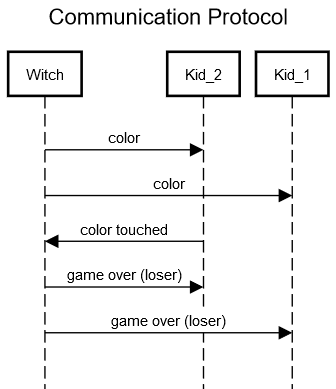
\includegraphics[width=0.7\textwidth]{images/CommunicationProtocol.png}
		\caption{Rappresentazione grafica del protocollo di comunicazione.}
		\label{fig:communicationprotocol}
	\end{figure}
		\newpage
		
	\section{Modulo di Visione}
		Il modulo inerente agli aspetti di computer vision è stato realizzato mediante l'uso di una telecamera RGB-D, in particolare tramite una {\itshape Microsoft Kinect}, il cui stream video è stato processato con l'ausilio dell'API {\itshape OpenCV}.\newline
Il modulo di visione in questione prevede la realizzazione della seguente pipeline:
\begin{enumerate}
	\item acquisizione dello stream video RGB e di profondità e conversione dello spazio di colore da RGB a HSV;
	\item ricerca del blob di massima dimensione del colore target associato alla sessione corrente;
	\item estrazione del valore di profondità associato al centroide del blob;
	\item calcolo del vettore in direzione del target.
\end{enumerate}
\subsection{Acquisizione dello stream video}
L'acquisizione dello stream video tramite camera RGB-D è stata realizzata mediante l'uso del framework open-source {\itshape OpenNI}, ideato per accedere alle informazioni registrate dalla camera con un livello di astrazione alto. In particolare, l'acquisizione dello stream video RGB è stata realizzata attraverso la sottoscrizione al topic \texttt {/camera/rgb/image\_rect\_color} mentre l'acquisizione dello stream video di profondità è stata realizzata attraverso la sottoscrizione al topic \\
\texttt {/camera/depth\_registered/image}.

Siccome entrambi i topic forniscono informazioni mediante messaggi di tipo \texttt{sensor\_msgs/Image}, per permettere l'analisi tramite {\itshape OpenCV} è necessario convertire entrambi gli stream video nel formato \texttt {cv::Mat}. La suddetta conversione è stata realizzata mediante l'uso della libreria {\itshape CvBridge} con la seguente funzione di conversione
\begin{center}
	\texttt{imgmsg\_to\_cv2(frame\_video, encoding)}
\end{center}
dove per encoding sono stati utilizzati \texttt{bgr8} ed \texttt{32FC1} rispettivamente per la conversione dell'immagine RGB e di profondità.

\begin{figure}[htbp]
	\begin{center}
		\subfigure[Frame RGB\label{fig:RGBimg}]{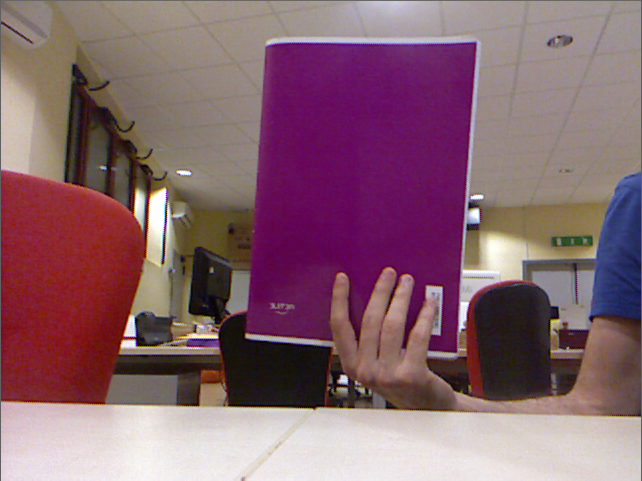
\includegraphics[width=55mm]{images/1-RGB.png}}
		\subfigure[Frame Depth\label{fig:depthImg}]{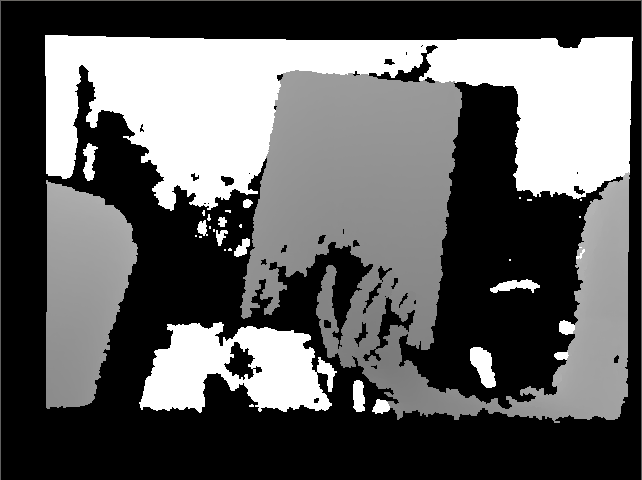
\includegraphics[width=55mm]{images/2-Depth.png}}
	\end{center}
\end{figure}

Per agevolare l'analisi dei frame è stato effettuato un preprocessing dei frame RGB in cui è prevista l'applicazione di un filtro gaussiano (per rimuovere l'eventuale presenza di rumore video) realizzato mediante l'uso di un kernel di dimensioni \texttt{3x3}. L'applicazione del suddetto filtro è stata ottenuta mediante l'uso della funzione \texttt{cv2.GaussianBlur()}.

Essendo questa fase fortemente soggetta ad una discriminazione dei colori presenti nei frame, è stata effettuata una conversione dello spazio di colori da \texttt{RGB} a \texttt{HSV} mediante la funzione \texttt{cv2.cvtColor()}. Così facendo viene gestita in maniera più "naturale" la distinzione dei colori, in quanto nello spazio HSV la variazione dei colori è soggetta soltanto alla componente {\itshape Hue} a differenza dello spazio RGB, in cui un colore viene visto come una combinazione di rosso, giallo e blu.

\subsection{Estrazione del blob e calcolo del centroide}
La {\itshape palette} dei colori a disposizione nel gioco è stata realizzata mediante l'uso di intervalli di colore espressi in formato HSV. Ad ogni colore quindi è associato un intervallo e durante la fase di estrazione del colore, ogni valore contenuto nell'intervallo associato al colore target è considerato valido.

Per realizzare tale selezione è stata utilizzata la funzione
\begin{center}
	\texttt{cv2.inRange(frame\_video, lower\_bound, upper\_bound)}
\end{center} 
dove per \texttt{lower\_bound} ed \texttt{upper\_bound} sono stati inseriti gli estremi dell'intervallo associati al colore target. Dalla funzione viene ritornata una maschera il cui scopo è di isolare dal frame corrente soltanto le informazioni utili alla ricerca del blob.

\begin{figure}[htbp]
	\begin{center}
		\subfigure[Maschera\label{fig:RGBimg}]{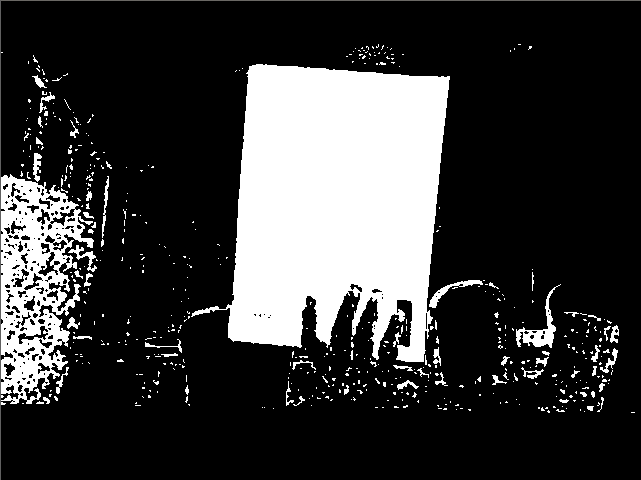
\includegraphics[width=55mm]{images/3-Mask.png}}
	\end{center}
\end{figure}

Tuttavia la maschera evidenzia anche piccole porzioni di immagine che possono deviare la corretta ricerca del blob e che quindi costituiscono un rumore. Per eliminare gran parte di tale rumore è stata effettuata un'operazione di {\itshape erosione} tramite l'uso della funzione \texttt{cv2.erode()} seguita da un'operazione di {\itshape dilatazione} tramite l'uso della funzione \texttt{cv2.dilate()} utile a ristabilire le proporzioni delle componenti utili evidenziate dalla maschera.

\begin{figure}[htbp]
	\begin{center}
		\subfigure[Erosione\label{fig:erosion}]{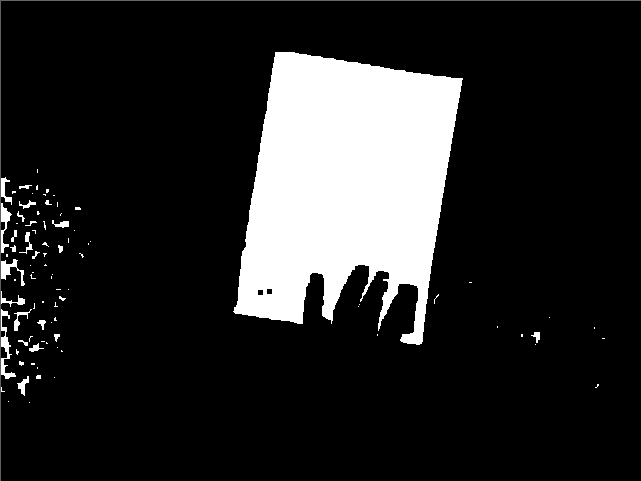
\includegraphics[width=55mm]{images/4-erode.png}}
		\subfigure[Dilatazione\label{fig:dilatation}]{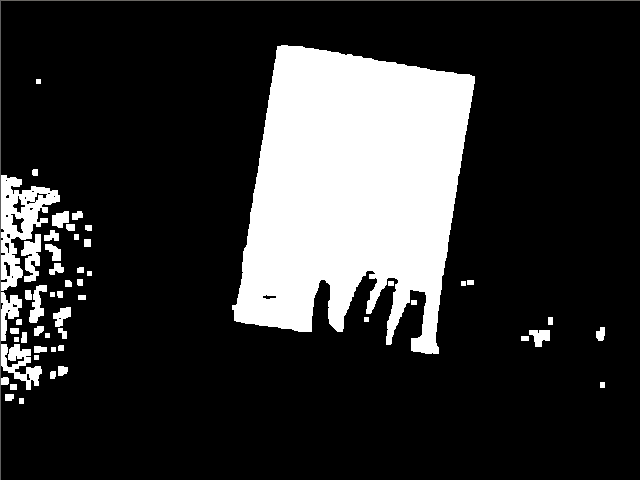
\includegraphics[width=55mm]{images/5-dilate.png}}
	\end{center}
\end{figure}

Per tener traccia dei blob presenti nella scena, è stata utilizzata la funzione
\begin{center}
	\texttt{cv2.findContours(mask, cv2.RETR\_EXTERNAL, cv2.CHAIN\_APPROX\_SIMPLE)}
\end{center}
dove \texttt{cv2.RETR\_EXTERNAL} indica che vengono estratti soltanto i contorni esterni (trascurando quindi i contorni innestati in altri), mentre \texttt{cv2.CHAIN\_APPROX\_SIMPLE} indica che viene realizzata un'ottimizzazione dello spazio necessario a memorizzare i contorni.

Successivamente viene selezionato il blob avente area maggiore e, tramite la funzione \texttt{cv2.minEnclosingCircle()}, viene estratto il raggio del cerchio di area minima che lo include. Il blob in questione viene considerato valido soltanto se avente raggio superiore ad una soglia fissata apriori.

Arrivati a questo punto, viene estratto il centroide mediante i {\itshape momenti dell'immagine} associati al contorno del blob tramite la funzione \texttt{cv2.moments(contour)}. In particolare, le coordinate che identificano il centroide sono così espresse:
\begin{center}
	$C_x=\frac{M_{10}}{M_{00}}$, $C_y=\frac{M_{01}}{M_{00}}$
\end{center}

\begin{figure}[htbp]
	\begin{center}
		\subfigure[Blob selezionato\label{fig:RGBimg}]{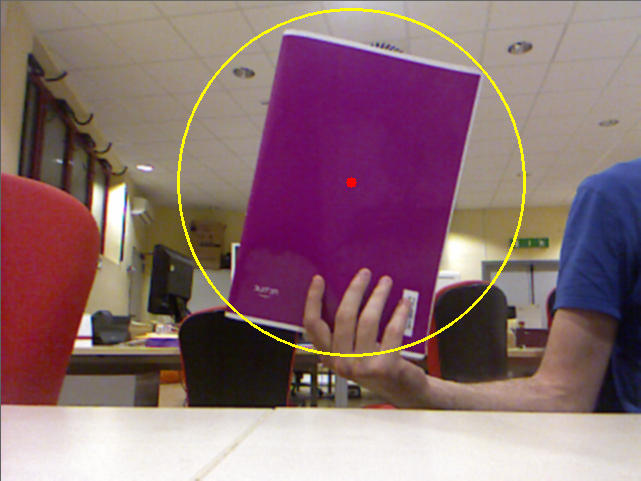
\includegraphics[width=55mm]{images/6-final.png}}
	\end{center}
\end{figure}

\subsection{Estrazione della profondità}
Giunti a questa fase, si ha a disposizione il centroide rappresentante il target da seguire. Possiamo quindi estrarre la distanza del blob dalla camera utilizzando la componente di profondità processata dalla camera RGB-D.

L'immagine di profondità a disposizione è nel formato \texttt{cv::Mat}, quindi per accedere alla distanza al centroide del blob è sufficiente estrarre dall'immagine la componente $(C_x,C_y)$. Così facendo si otterrà un valore in {\itshape floating point} a 32 bit rappresentante la distanza in metri del punto osservato nel pixel dalla camera.

\subsection{Calcolo della direzione da seguire}
Per ottenere il vettore in direzione del target è stato utilizzato il raggio uscente dalla camera ed entrante nel pixel che costituisce il centroide del target.\newline
Essendo l'immagine ottenuta per proiezione prospettica della scena visualizzata dalla camera su di un piano di proiezione, il raggio ottenuto potrà essere considerato valido per la generazione del vettore direzionale che vogliamo realizzare.

È stato utilizzato quindi il modello della {\itshape Pin-hole camera} per elaborare le informazioni associate alla Kinect ed estrarre il raggio in questione. Tali informazioni vengono estratte dal topic \texttt{/camera/depth\_registered/camera\_info} sottoforma di messaggio \texttt{sensor\_msgs/CameraInfo}.
Il modello della camera viene realizzato mediante l'uso dell'oggetto \texttt{PinholeCameraModel} contenuto nella libreria \texttt{image\_geometry} nativa di ROS.
Successivamente, mediante la funzione
\begin{center}
	\texttt{projectPixelTo3dRay(centroid)}
\end{center}
viene estratto il raggio uscente dalla camera in direzione della coppia di coordinate $C_x,C_y$ sottoforma di versore. Infine, dalla moltiplicazione delle componenti $x,z$ del raggio appena ottenuto con la distanza estratta allo step precedente, viene generato il vettore direzionale utile al robot per raggiungere il target.

		\newpage
		
	\section{Dettagli Implementativi}
		% RoleManager
		% il fatto che "vediamo" solo ogni mezzo secondo
		% problemi: sonar che rimbalzano
		%	DETTAGLI IMPLEMENTATIVI

\subsection{Role Manager}
	La gestione dei ruoli avviene in modo dinamico: ogni volta che inizia un nuovo turno, il robot sa quale roulo dovr� ricoprire. Tale gestione � demandata interamente alla classe \texttt{RoleManager}, la quale � responsabile di:
	\begin{itemize}
		\item settaggio parametri;
		\item lancio dei nodi Kid e Witch;
		\item creazione e connessione delle socket;
		\item gestione dei messaggi.
	\end{itemize}
	Al primo avvio, il sistema impone che il primo robot a ricoprire il ruolo di Witch sia quello con indirizzo IP minore rispetto a tutti gli altri. Per tutti gli altri match, il Role Manager del robot perdente lancia il nodo Witch e tutti gli altri quello Kid.

\subsection{Problemi Relativi alla Sensoristica}
	Durante la fase di test sono state individuate due principali problematiche relative alla sensoristica dei robot: una riguardante i sonar e l'altra la telecamera.
	Per quanto riguarda i sonar, sono stati riscontrati i classici problemi di riflessione delle onde a ultrasuoni. Infatti, utilizzando uno scatolo quadrato come ostacolo, nel momento in cui il robot di muove in direzione di un suo spigolo, i sonar non riescono ad individuare l'ostacolo in quanto le onde emesse vengono riflesse altrove, non ritornando al sensore. Per quanto riguarda invece il problema del \textit{cross-talk}, � stato riscontrato ma raramente.
	
	Le problematiche relative alla telecamera RGB-D riguardano i valori di profondit� per oggetti a distanza minore di $\simeq 0.5$ e il tempo di elaborazione dei frames. Per tali oggetti infatti la distanza calcolata dalla telecamera risulta avere valore \texttt{NaN}. Il problema � stato gestito utilizzando una stima della posizione del POI precedentemente rilevata: quando la misurazione � \texttt{NaN}, ma il POI si trova ad una distanza stimata limite, l'oggetto viene riconosciuto come "toccato".
	Al fine di rendere il movimento del robot pi� fluido, si � deciso di richiamare la funzione di elaborazione dell'immagine con cadenza regolare poich� l'elevato tempo di elaborazione diminuiva la frequenza di esecuzione del loop di controllo. Ci� causava movimenti troppo lunghi che, in situazioni critiche, a condizioni di stallo.
	
\end{document}
